\documentclass[12pt,a4paper]{article}
\usepackage[margin=1in]{geometry}
\usepackage{setspace}
\usepackage{graphicx}
\usepackage{amsmath}
\usepackage{enumitem}
\usepackage{float}
\usepackage{graphicx}
\usepackage{fancyhdr}
\usepackage{hyperref} % clickable URLs
\setlength{\headheight}{2cm}
\setlength{\headsep}{0.5 cm}
\newcommand{\subjectname}{Advanced Data Structures and Algorithms (DJS23APE302)}
\onehalfspacing
\pagestyle{fancy}
\fancyhf{} % clear default header/footer
\fancyhead[C]{\includegraphics[width=0.9\textwidth,height=2.5cm,keepaspectratio]{college_header.JPG}}
\fancyfoot[L]{\textbf{Subject:} \subjectname}
\fancyfoot[R]{\thepage}
\begin{document}
\begin{center} 
    \large \textbf{Department of Artificial Intelligence and Machine Learning}\\
    \Large \textbf{Experiment No.: 2} \\
    \large \textbf{To perform and implement Hiring Problem..}
\end{center}

\section*{Aim}
To perform and implement the Hiring Problem algorithm and analyze its performance.

\subsection*{Learning Objectives}

After completing this experiment, students will be able to:

\begin{itemize}
    \item Understand and implement the Hiring Problem algorithm.
    \item Explain the concept of probabilistic analysis.
    \item Understand the importance of randomized algorithms in optimization problems.
\end{itemize}
\section*{Theory}

The \textbf{Hiring Problem} is a classical algorithm used to explain the concepts of probabilistic analysis and randomized algorithms.A company interviews $n$ candidates one by one in a random order. After each interview, an immediate decision must be made whether to hire the candidate. The hiring strategy is as follows:

\begin{itemize}
    \item Hire the first candidate.
    \item For every subsequent candidate:
    \begin{itemize}
        \item Compare the candidate with the currently hired candidate.
        \item If the new candidate is better, hire the candidate and replace the current employee.
        \item Otherwise, reject the candidate.
    \end{itemize}
\end{itemize}

The objective is to ensure that the best candidate is hired while minimizing the number of hiring decisions.

\subsection*{Algorithm}

\begin{enumerate}
    \item Read the list of candidates.
    \item Hire the first candidate.
    \item Assume the first candidate as the current best.
    \item Traverse the remaining candidates.
    \item Compare each candidate with the current best.
    \item If the current candidate is better:
    \begin{itemize}
        \item Hire the candidate.
        \item Update the current best.
    \end{itemize}
    \item Display the best candidate and the total number of hiring decisions.
\end{enumerate}

\subsection*{Problem Statement}
1. There are n workers. You are given two integer arrays quality and wage where quality[i] is the quality of the ith worker and wage[i] is the minimum wage expectation for the ith worker.
We want to hire exactly k workers to form a paid group. To hire a group of k workers, we must pay them according to the following rules:
\begin{itemize}
\item Every worker in the paid group must be paid at least their minimum wage expectation.
\item In the group, each worker's pay must be directly proportional to their quality. This means if a worker’s quality is double that of another worker in the group, then they must be paid twice as much as the other worker.
\end{itemize}
Given the integer k, return the least amount of money needed to form a paid group satisfying the above conditions. Answers within 10-5 of the actual answer will be accepted.
\begin{figure}[H]
    \centering
    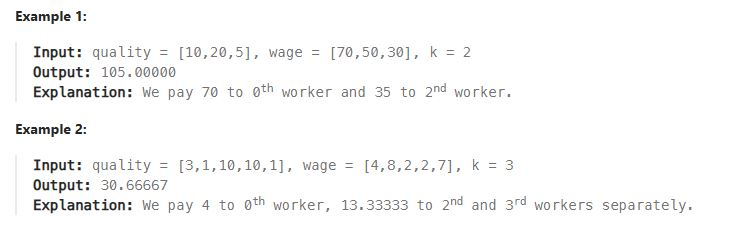
\includegraphics[width=0.8\linewidth]{exp 2.JPG}
\end{figure}

2. You are given a \textbf{0-indexed} integer array \texttt{costs} where
\texttt{costs[i]} is the cost of hiring the $i^{th}$ worker.You are also given two integers \texttt{k} and \texttt{candidates}.
We want to hire exactly \texttt{k} workers according to the following rules:
\begin{itemize}
    \item You will run \texttt{k} sessions and hire exactly one worker in each session.
    \item In each hiring session, choose the worker with the lowest cost from either the first
    \texttt{candidates} workers or the last \texttt{candidates} workers.
    Break the tie by the smallest index.
    \begin{itemize}
        \item For example, if
        \texttt{costs = [3,2,7,7,1,2]} and
        \texttt{candidates = 2},
        then in the first hiring session, we will choose the $4^{th}$ worker because they have the
        lowest cost \texttt{[3,2,7,7,\textbf{1},2]}.
        \item In the second hiring session, we will choose the $1^{st}$ worker because they have the same
        lowest cost as the $4^{th}$ worker, but they have the smaller index
        \texttt{[3,2,7,2]}.
        Please note that the indexing may be changed in the process.
    \end{itemize}
    \item If there are fewer than \texttt{candidates} workers remaining, choose the worker with the
    lowest cost among them. Break the tie by the smallest index.
    \item A worker can only be chosen once.
\end{itemize}
Return the \textit{total cost to hire exactly} \texttt{k} \textit{workers}.
\begin{figure}[H]
     \centering
     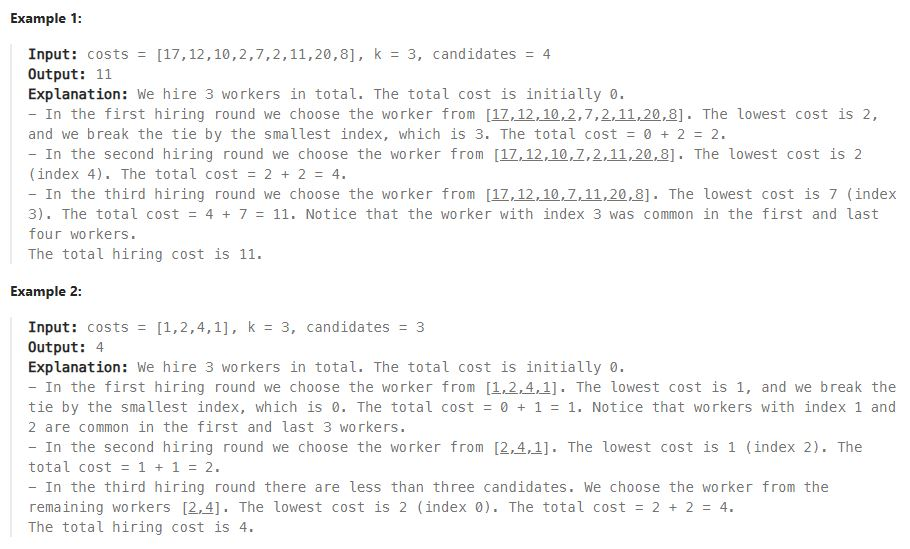
\includegraphics[width=1\linewidth]{example 2.JPG}
 \end{figure} 
 %%%%%%%%%%%%%%%%%%%%%%%%%%%%%%%%%%%%%%%%%%%%%%%%%%%%%%%%%%%%
\subsection*{Viva Questions}

\begin{enumerate}
    \item What is the Hiring Problem?
    
    \item Why is the Hiring Problem considered a probabilistic algorithm?
    
    \item What is the objective of the Hiring Problem?
            
    \item What is meant by a hiring cost?
    
    \item What is the difference between interview cost and hiring cost?
           
    \item What is the expected number of hires if the candidates arrive in random order?
    \item Why is randomization useful in the Hiring Problem?
    
    \item What is the worst-case scenario for the Hiring Problem?
    
    \item What is the best-case scenario for the Hiring Problem?
   
\end{enumerate}

%%%%%%%%%%%%%%%%%%%%%%%%%%%%%%%%%%%%%%%%%%%%%%%%%%%%%%%%%%%%
\subsection*{References}

\begin{enumerate}
    \item Thomas H. Cormen, Charles E. Leiserson, Ronald L. Rivest, and Clifford Stein, \textit{Introduction to Algorithms}, 4th Edition, MIT Press, 2022.    
      
    \item Alfred V. Aho, John E. Hopcroft, and Jeffrey D. Ullman, \textit{The Design and Analysis of Computer Algorithms}, Pearson Education.    
       
    \item MIT OpenCourseWare, \textit{Introduction to Algorithms}. Available at: \texttt{https://ocw.mit.edu}  
   
\end{enumerate}
%%%%%%%%%%%%%%%%%%%%%%%%%%%%%%%%%%%%%%%%%%%%%%%%%%%%%%%%%%%%
\end{document}

